\pgfplotstablegetelem{\thepart}{[index]\columnIndex}\of{\cronograma}
\part{\pgfplotsretval}
\label{part:\thepart}
\frame{\partpage}



\begin{frame}[t]{Uso e declaração dos métodos}
	
	\fontsize{14pt}{15}\selectfont{
		...continuando \acrshort{poo}.\\ 
		
		Quando o método é declarado sempre o primeiro parâmetro é self, quando é necessário acesso ao objeto.	Entretanto nas chamadas omite-se esse parâmetro. O correspondente ao self torna-se o prefixo da chamada.
		
	}\par
	\vspace{1em}
	
	
	Declaração:
	\vspace{1em}
	\begin{beamercolorbox}[wd=\textwidth]{warning}		
		def altera\_preco(self, novo\_preco):\\
		\hspace{1em}{Instruções}
	\end{beamercolorbox}

	Uso:
	\vspace{1em}
	\begin{beamercolorbox}[wd=\textwidth]{warning}
		p1 = Produto("Arroz", 1, 2, 5)\\
		if p1.altera\_preco(2): print('False')
	\end{beamercolorbox}
	
	
\end{frame}



\begin{frame}[t]{O método construtor}
	
	\fontsize{14pt}{15}\selectfont{
		
		\textbf{\_\_init\_\_} é um método especial dentro da classe. É construtor da classe, onde os atributos do objeto recebem seus valores iniciais. 
		
	}\par
	\vspace{1em}
	
	
	\fontsize{12pt}{15}\selectfont{
		\begin{itemize}%[<+->] 
			
			\item No caso da classe acima, os 4 atributos (variáveis) que caracterizam um produto, recebem neste método seus valores iniciais, que podem ser modificados por operações futuras deste mesmo objeto. 
			
			\item A criação de um novo produto, ou seja, a criação de uma instância do objeto produto causa a execução do método \textbf{\_\_init\_\_}. Assim, o comando abaixo, causa a execução do método \textbf{\_\_init\_\_}:
			
			
			\vspace{1em}
			\begin{beamercolorbox}[wd=\textwidth]{warning}
				p1 = Produto("Arroz", 1, 2, 5)
			\end{beamercolorbox}
			
		\end{itemize}
	}\par
	\vspace{1em}
	
\end{frame}



\begin{frame}[t]{Explorar a sintaxe das classes – o parâmetro self}
	
	\fontsize{14pt}{15}\selectfont{
		
		O parâmetro self é importante no método construtor da classe \textbf{\_\_init\_\_}, para referenciar o objeto que está sendo criado. Nos demais métodos, se usado, é simplesmente um parâmetro. Nem precisa ser o primeiro. Mesmo no \textbf{\_\_init\_\_}, o primeiro parâmetro pode ter qualquer nome. 
		
	}\par
	\vspace{1em}
	
	\fontsize{14pt}{25}\selectfont{
		\begin{beamercolorbox}[wd=\textwidth]{warning}
			class Produto:\\
			\hspace{1em}def \_\_init\_\_(outro, nome):\\
			\hspace{2em}outro.nome = nome\\
			
			
			\hspace{1em}def altera\_nome(nome, self):\\
			\hspace{2em}self.nome = nome
		\end{beamercolorbox}
		
	}\par
	\vspace{1em}
	
\end{frame}




\begin{frame}[t]{Explorar a sintaxe das classes – o parâmetro self}
	
	
	
	\fontsize{12pt}{15}\selectfont{
		\begin{itemize}%[<+->] 
			
			\item No caso da classe acima, os 4 atributos (variáveis) que caracterizam um produto, recebem neste método seus valores iniciais, que podem ser modificados por operações futuras deste mesmo objeto. 
			
			\item A criação de um novo produto, ou seja, a criação de uma instância do objeto produto causa a execução do método \textbf{\_\_init\_\_}. Assim, o comando abaixo, causa a execução do método \textbf{\_\_init\_\_}:
			
			
			\vspace{1em}
			\begin{beamercolorbox}[wd=\textwidth]{warning}
				p1 = Produto("Arroz", 1, 2, 5)
			\end{beamercolorbox}
			
		\end{itemize}
	}\par
	\vspace{1em}
	
\end{frame}



\begin{frame}[t]{Explorar a sintaxe das classes}
	
	\fontsize{14pt}{15}\selectfont{
		
		Uma classe não precisa necessariamente ter um método construtor. Podemos ter uma classe apenas com métodos, sem atributos. Nesse caso, o nome da classe é usado sem parâmetros para a chamada das funções.
		
	}\par
	\vspace{1em}
	
	\fontsize{14pt}{25}\selectfont{
		\begin{beamercolorbox}[wd=\textwidth]{warning}
			class Produto:\\		
			
			\hspace{1em}def imprime\_nome(nome):\\
			\hspace{2em}print(nome)\\
			\vspace{1em}
			Produto.imprime\_nome('Arroz')
			
		\end{beamercolorbox}
		
	}\par
	\vspace{1em}
	
\end{frame}



\begin{frame}[t]{Herança em classes}
	
	\fontsize{14pt}{15}\selectfont{
		
		Permite que uma classe seja definida com base em classe já existente. Dizemos que essa nova classe herda características da classe original. 
		
	}\par
	\vspace{1em}
	
	\fontsize{12pt}{15}\selectfont{
		\begin{itemize}%[<+->] 
			
			\item Na terminologia Python a classe original é chamada de Classe Base, Classe Mãe ou Superclasse (Base, Parent ou Super Class) enquanto que a nova é chamada de Sub Classe ou Classe Filha (Sub ou Child Class).
			
			\item A subclasse pode especializar a classe principal ou mesmo estendê-la com novos métodos e atributos.
			
		\end{itemize}
	}\par
	\vspace{1em}
	
\end{frame}





\begin{frame}[t]{Herança em classes}
	
	\fontsize{14pt}{15}\selectfont{
		
		Uma classe não precisa necessariamente ter um método construtor. Podemos ter uma classe apenas com métodos, sem atributos. Nesse caso, o nome da classe é usado sem parâmetros para a chamada das funções.
		
	}\par
	\vspace{1em}
	
	\fontsize{14pt}{25}\selectfont{
		\begin{beamercolorbox}[wd=\textwidth]{warning}
			class Produto:\\		
			
			\hspace{1em}def imprime\_nome(nome):\\
			\hspace{2em}print(nome)\\
			\vspace{1em}
			Produto.imprime\_nome('Arroz')
			
		\end{beamercolorbox}
		
	}\par
	\vspace{1em}
	
\end{frame}



\begin{frame}[t]{Herança em classe}	
	
	\lstinputlisting[style=CBruno,caption=Herança da classe Produto]{outros/codigos/python/codigo_004_classe_produto_critico.py}
	
	
	*obs: \textbf{class ProdutoCritico(Produto)} é uma classe derivada de Produto: indica que \textbf{ProdutoCritico} é uma subclasse da classe \textbf{Produto}.
	
\end{frame}

\begin{frame}[t]{Pytest}
	
	\vspace{-1em}
	\lstinputlisting[style=CBruno,caption=Cobertura de testes da classe Produto Crítico]{outros/codigos/python/test_codigo_004_classe_produto_critico.py}
	
	
\end{frame}



\begin{frame}[t]{Pytest}
	
	
	\vspace{1em}
	\centering
	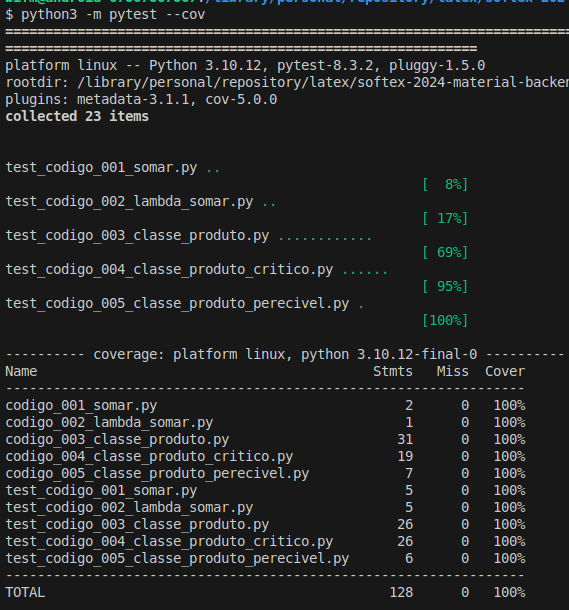
\includegraphics[scale=0.3]{imagens/fig-result-test-produto-critico.png}
	
\end{frame}





\begin{frame}[t]{Polimorfismo em classe}
	
	\fontsize{14pt}{15}\selectfont{
		
		Polimorfismo permite que objetos de diferentes classes sejam tratados como objetos de uma classe comum.
		
	}\par
	\vspace{1em}
	
	\fontsize{12pt}{15}\selectfont{
		\begin{itemize}%[<+->] 
			
			\item Polimorfismo é o princípio pelo qual duas ou mais classes derivadas de uma mesma superclasse podem invocar métodos que têm a mesma identificação, assinatura, mas comportamentos distintos, especializados para cada classe derivada, usando para tanto uma referência a um objeto do tipo da superclasse.
			
			%			\item 
			
		\end{itemize}
	}\par
	\vspace{1em}
	
\end{frame}






\begin{frame}[t]{Polimorfismo em classe}	
	
	\lstinputlisting[style=CBruno,caption=Polimorfismo de classe]{outros/codigos/python/codigo_005_classe_produto_perecivel.py}
	
	\vspace{1em}
	
	*obs: \textbf{class ProdutoPerecivel(Produto)} é uma classe derivada de Produto: indica que \textbf{ProdutoPerecivel} é uma subclasse da classe \textbf{Produto}.
	
\end{frame}

\begin{frame}[t]{Pytest}
	
	%	\vspace{-2em}
	\lstinputlisting[style=CBruno,caption=Cobertura de testes da classe Produto Perecivel]{outros/codigos/python/test_codigo_005_classe_produto_perecivel.py}
	
	
\end{frame}




\begin{frame}[t]{Pytest}
	
	\centering
	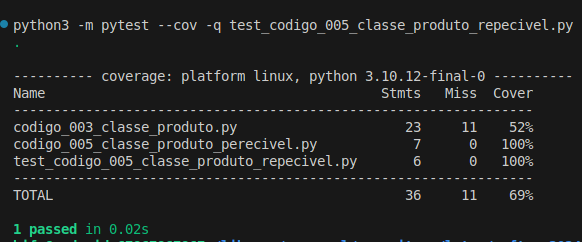
\includegraphics[scale=0.5]{imagens/fig-result-test-especifico-produto-perecivel.png}
	
\end{frame}


\begin{frame}[t]{Pytest}
	
	\centering
	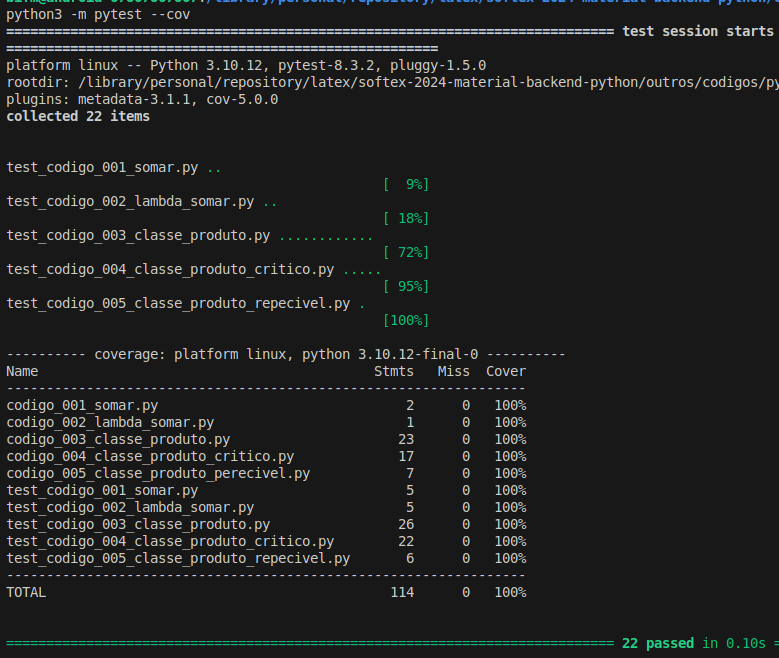
\includegraphics[scale=0.3]{imagens/fig-result-test-produto-perecivel.png}
	
\end{frame}






\begin{frame}[t]{Polimorfismo em classe}	
	
	\fontsize{14pt}{15}\selectfont{
		
		Sobreposição.
		
	}\par
	\vspace{1em}
	
	\fontsize{12pt}{15}\selectfont{
		\begin{itemize}%[<+->] 
			
			%			\item Sobrecarga (Overload): é o ato de criar vários métodos diferentes com o mesmo o nome, porém com assinaturas diferentes, cada um com sua própria implementação. Python não trabalha com overload por padrão. Para alcançar é possível utilizar bibliotecas com decoratores.
			
			\item Sobreposição (Override): é sobrescrever, ou seja, definir um novo comportamento para um método que já existe. Isso acontece quando a classe em questão herda (estende) outra classe e se cria um método com a mesma assinatura da classe "pai" na classe filha.
			
		\end{itemize}
	}\par
	\vspace{1em}
	
\end{frame}



\begin{frame}[t]{Encapsulamento em classe}
	
	\fontsize{12pt}{15}\selectfont{
		
		Encapsulamento é a proteção dos atributos ou métodos de uma classe, em Python existem somente o public e o private e eles são definidos no próprio nome do atributo ou método.
		
	}\par
	
	\vspace{0.5em}
	\fontsize{8pt}{10}\selectfont{
		\begin{beamercolorbox}[wd=\textwidth]{warning}
			class Veiculo:\\
			\hspace{1em}chassi = 1 \# atributo publico\\
			\hspace{1em}\_\_motor = 2 \# atributo privado a classe Veiculo. O símbolo \_\_* define como privado.\\
			\vspace{0.5em}
			class Carro(Veiculo):\\
			\hspace{1em}\_\_placa = 3 \# atributo privado a classe Carro\\
			\vspace{0.5em}
			\hspace{1em}def \_\_init\_\_(self):\\
			\hspace{2em}print(self.chassi)\\
			\hspace{2em}print(self.\_\_placa)\\
			\vspace{0.5em}
			veiculo = Veiculo()\\
			print(veiculo.chassi) \# imprime 1\\
			\vspace{0.5em}
			carro = Carro() \# Erro\\
			\# print(carro.\_\_motor) \# Erro, pois \_\_motor é privado a classe Veiculo.\\
			\# print(carro.\_\_placa) \# Erro, \_\_placa é um atributo privado, somente chamado pela classe Carro.\\
		\end{beamercolorbox}
		
	}\par
	\vspace{1em}
	
	
\end{frame}






\begin{frame}[t]{Encapsulamento em classe}
	
	\begin{block}{Exemplo anteior}		
		class Veiculo:\\
		\hspace{1em}chassi = 1 \# atributo publico\\
		\hspace{1em}\_\_motor = 2 \# atributo privado a classe Veiculo. O símbolo \_\_* define como privado.\\
		\vspace{0.5em}
		class Carro(Veiculo):\\
		\hspace{1em}\_\_placa = 3 \# atributo privado a classe Carro\\
		\vspace{0.5em}
		\hspace{1em}def \_\_init\_\_(self):\\
		\hspace{2em}print(self.chassi)\\
		\hspace{2em}print(self.\_\_placa)\\
		\vspace{0.5em}
		veiculo = Veiculo()\\
		print(veiculo.chassi) \# imprime 1\\
		\vspace{0.5em}
		carro = Carro() \# Erro\\
		\# print(carro.\_\_motor) \# Erro, pois \_\_motor é privado a classe Veiculo.\\
		\# print(carro.\_\_placa) \# Erro, \_\_placa é um atributo privado, somente chamado pela classe Carro.\\
	\end{block}
	
	
\end{frame}




\begin{frame}[t]{Tratamento de exceções}
	
	\fontsize{13pt}{15}\selectfont{
		
		O tratamento de exceção, na ciência da computação, é o mecanismo responsável pelo tratamento da ocorrência de condições que alteram o fluxo normal da execução de programas de computadores. \\Para condições consideradas parte do fluxo normal de execução, ver os conceitos de sinal e evento.
		
	}\par
	
	\vspace{2em}
	Saiba mais em
	\url{https://docs.pytest.org/en/stable/how-to/assert.html}
	
\end{frame}







\begin{frame}[t]{Tratamento de exceções}
	
	\vspace{1em}
	
	\fontsize{13pt}{15}\selectfont{
		A sintaxe básica é:		
	}\par
	
	\vspace{1em}
	\begin{beamercolorbox}[wd=\textwidth]{warning}
		try: \\
		\hspace{1em}{Instruções} \# o código da funcionalidade.\\
		...\\
		except <ExceptType>:\\
		\hspace{1em}{Instruções} \# o código para tratamento da exceção.\\
		...\\
		finally: \# Caso o fluxo não seja interrompido, sempre é executado o finally.\\
		\hspace{1em}{Instruções}
	\end{beamercolorbox}
	
	
	\vspace{2em}
	\url{https://docs.python.org/pt-br/3/tutorial/errors.html}
	
\end{frame}














\begin{frame}[t]{Tratamento de exceções}	
	
	\lstinputlisting[style=CBruno,caption=Tratamento de exceções]{outros/codigos/python/codigo_006_classe_veiculo_com_exception.py}
	
	
\end{frame}





\begin{frame}[t]{Pytest}
	
	%	\vspace{-2em}
	\lstinputlisting[style=CBruno,caption=Cobertura de testes da classe Veiculo]{outros/codigos/python/test_codigo_006_classe_veiculo_com_exception.py}
	
	
\end{frame}


